% Chapter Template

\chapter{Supercharging our Numerical Methods}

\label{Chapter5} % Change X to a consecutive number

\lhead{Chapter 5. \emph{Faster Computations with Parareal}}
\section{Parareal}
    The hunger for speed and accuracy can't be satisfied without using all our computer's resource to crunch the numbers. The most obvious way to do this is is to run our code on separate threads concurrently. 
    
\subsection{Algorithm Description}
The Parareal Algorithm follows these steps:
\begin{enumerate}
    \item Compute a "bad" approximation to the solution using the coarse solver.
    \item Compute corrections in parallel using the fine solver.
    \item Update the solution iteratively using a predictor-corrector approach until convergence is achieved.
\end{enumerate}

\subsection{Mathematical Formulation}
Consider a differential equation of the form:
\begin{equation}
    \frac{du}{dt} = f(u,t), \quad u(0) = u_0.
\end{equation}
The time domain is divided into intervals, and two solvers are defined:
\begin{itemize}
    \item A coarse solver, $C_j^k$, which provides an initial guess.
    \item A fine solver, $F_j^k$, which refines the solution in parallel.
\end{itemize}
The iteration formula is given by:
\begin{align*}
    C_{j+1}^{k+1} = C_{j+1}^k + F_j^k - C_j^k.
\end{align*}
The method is captured beautifully by this 
\href{https://upload.wikimedia.org/wikipedia/commons/transcoded/b/b5/Parareal_Animation.ogv/Parareal_Animation.ogv.720p.vp9.webm}{animation} from Wikipedia.
\subsection{Benchmarks}
The source code and benchmarking code is written in GoLang.
The following results are taken when the baseline RK4 solution runs with 1,00,000 iterations while the Parareal solution runs with 1000 coarse steps and 200 fine sub-steps. So the Parareal solution computes 2X the number of points.
\newpage
\begin{verbatim}
go test -bench .  
goos: linux
goarch: amd64
pkg: example.com/greetings
cpu: AMD Ryzen 7 7730U with Radeon Graphics         
BenchmarkParareal-16                  84          14755702 ns/op
BenchmarkRK4-16                        2         745605400 ns/op
PASS
ok      example.com/greetings   3.482s
\end{verbatim}
This shows that the baseline RK4 method performs $\frac{745605400 }{14755702} \approx 50$ times slower !!
\begin{figure}
    \centering
    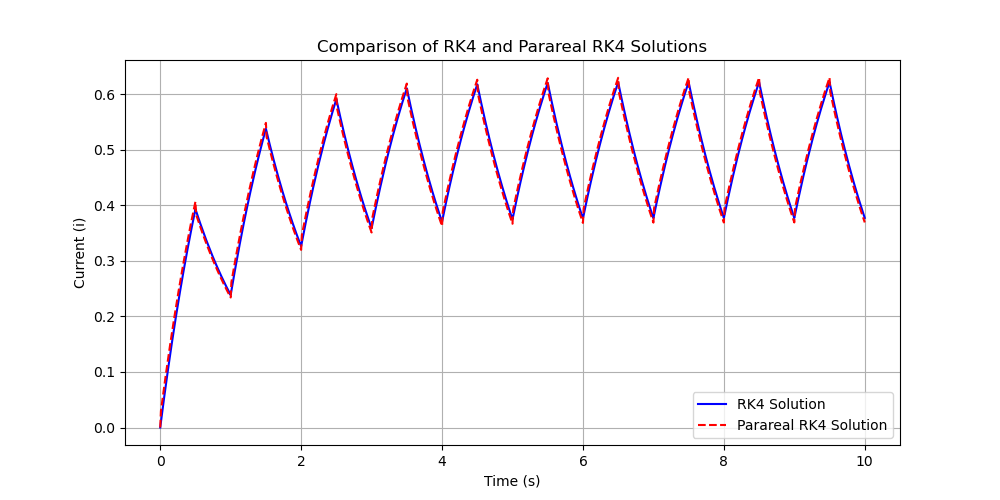
\includegraphics[width=0.8\linewidth]{figs/benchmark.png}
    \caption{Parareal v.s RK4}
\end{figure}